
\subsection{Schubmittelpunkt}
\subsubsection{Theorie}
Text folgt
\subsubsection{Berechnung}
Für die Berechnung des Schubmittelpunkts wird das Flügelprofil als vereinfachter Mehrzeller angenommen.
Dabei wird der Ursprung des Koordinatensystems am unteren rechten Rand gesetzt. Das Modell wird in 10 Teilstrecken $s_{i}$ aufgeteilt. Die Dicke wird über die Schale konstant angenommen und die Dicke des Stegs wird mit $t_{1}=1,882\mathrm{mm}$ angenommen, sowie die Dicke der Gurte mit $\mathrm{D}=1,941\mathrm{mm}$.
\begin{figure}[h]
 \centering
 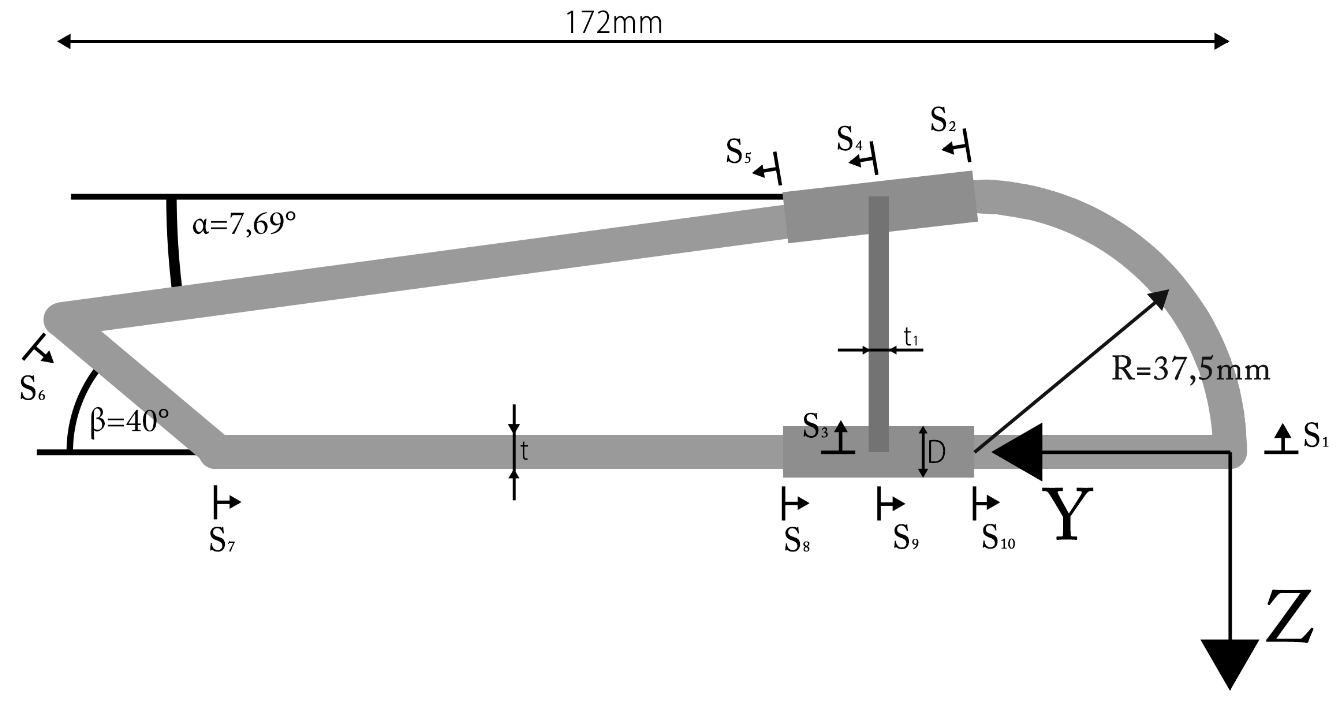
\includegraphics[width=0.7\textwidth]{Bilder/Model1}
 \caption{vereinfachtes Model}
 \label{fig:Model1}
\end{figure}

Zunächst werden die statischen Momente in den einzelnen Teilstücken berechnet.
\begin{equation}
	S_{z}=\int_{A}^{}y \mathrm{d}A =t\int_{s}^{}y \mathrm{d}s
\end{equation}
\begin{equation}
	S_{y}=\int_{A}^{}z \mathrm{d}A =t\int_{s}^{}z \mathrm{d}s 
\end{equation}
Damit ergeben sich für die statischen Momente:

\begin{center}
\begin{tabular}[h]{l|c|c}
	
Bauteilabschnitt&$S_{y}$&$S_{z}$\\
\hline
1& -1406,25&802,6823346\\
2&-1505,45762&1829,650931\\
3&-1323,28125&3627,555\\
4&-1428,32286&2400,902794\\
5&-2859,540449&12778,1555\\
6&-290,6472468&4825,70943\\
7&0&8949,4158\\
8&0&2408,679\\
9&0&1832,243\\
10&0&703,125\\
\end{tabular}
\end{center}

\noindent Nun kann aus den statischen Momenten der Schwerpunkt bestimmt werden:
\begin{equation}
	y_{0}=\frac{\int_{s}{}t(s)y\mathrm{d}s}{\int_{s}{}t(s)\mathrm{d}s}=\frac{S_{z}}{A}
\end{equation}
\begin{equation}
	y_{0}=\frac{\int_{s}{}t(s)z\mathrm{d}s}{\int_{s}{}t(s)\mathrm{d}s}=\frac{S_{y}}{A}
\end{equation}
Mit einer Dicke von $t=1\mathrm{mm}$ ergeben sich Lagen der Schwerpunktkoordinaten zu:
\begin{equation}
	y_{0}=180,94mm
\end{equation}
\begin{equation}
	z_{0}=-32,60mm
\end{equation}

Damit können nun die statischen Momente im Bezug auf den Schwerpunkt ermittelt werden:
\begin{center}
\begin{tabular}[h]{l|c|c}
Bauteilabschnitt&$S_{\bar{y}}$&$S_{\bar{z}}$\\
\hline
1&-467,32&-3475,48\\
2&-849,15&-1160,75\\
3&-198,33&-1498,19\\
4&-772,01&-589,50\\
5&-1142,51&4954,62\\
6&188,66&2641,77\\
7&1330,33&2887,85\\
8&656,30&-581,72\\
9&656,30&-1158,16\\
10&597,74&-2020,44\\
\end{tabular}
\end{center}
Für ein offenes Profil muss gelten, dass an der Schnittstelle das statische Moment $ 0 $ ist. Das Profil wird in diesem Fall an der Stelle 1 geschnitten.Die Verrechnung der statischen Momente ergibt 0, wodurch die statischen Momente als richtig angenommen werden können.


Nun müssen die Flächenträgheitsmomente $I_{y}$, $I_{z}$und $I_{zy}$ mit dem Drehwinkel $\alpha$ , sowie die schwerpunktbezogenen Flächenträgheitsmomente $I_{\bar{y}}$, $I_{\bar{z}}$ und $I_{\bar{zy}}$ mit Hilfe des Steiner-Anteils, ermittelt werden.Dafür werden die Winkelverschiebungen zum Koordinatensystem verwendet.
Es ergibt sich:
\begin{center}

\begin{tabular}[h]{l|c|c|c||c|c|c}
Bauteilabschnitt&$I_{y}$&$I_{z}$&$I_{zy}$&$I_{\bar{y}}$&$I_{\bar{z}}$&$I_{\bar{zy}}$\\
\hline
1&14288,06&14288,06&703,13&29254,35&86976,91&-32279,94\\
2&41,19&660,99&85,25&17553,77&33384,13&24024,05\\
3&8270,51&20,83&0&8827,87&31825,09&4210,30\\
4&41,19&660,99&85,25&14516,69&9101,00&11138,45\\
5&1873,93&102296,68&13811,66&13991,74&330186,63&-38738,58\\
6&937,64&1330,65&-1114,45&2121,31&233421,36&15460,20\\
7&6,96&48445,55&0&21212,10&148369,78&46031,60\\
8&29,68&672,51&0&10490,99&8891,32&-9272,51\\
9&29,68&672,51&0&10490,99&33249,65&-18460,76\\
10&3,13&4394,53&0&9530,96&113252,59&-32205,30\\
\hline
$\sum{}$&-&-&-&137990,78&1028658,46&-30092,48
\end{tabular}
\end{center}
Für das offene Profil lässt sich die Lage des Schubmittelpunkts nun mit folgenden Gleichungen bestimmen:
\begin{equation}
	y_{M}=\frac{-I_{\bar{z}}\int S_{\bar{y}}(s) r_{t}\mathrm{d}s+I_{\bar{yz}}\int S_{\bar{z}}(s) r_{t}\mathrm{d}s}{I_{\bar{y}}I_{\bar{z}}-I_{\bar{yz}}^2}
\end{equation}
\begin{equation}
	z_{M}=\frac{-I_{\bar{yz}}\int S_{\bar{y}}(s) r_{t}\mathrm{d}s+I_{\bar{y}}\int S_{\bar{z}}(s) r_{t}\mathrm{d}s}{I_{\bar{y}}I_{\bar{z}}-I_{\bar{yz}}^2}
\end{equation}
Daraus folgt:
\begin{equation}
	y_{M}=180,94mm
\end{equation}
\begin{equation}
	z_{M}=-32,60mm
\end{equation}
Nun muss der Schubmittelpunkt für das geschlossene Profil berechnet werden. Die Formeln dafür lauten:
\begin{equation}
	z_{M_{g}}=
	\frac{2\cdot A_{0}}{I_{\bar{y}}I_{\bar{z}}-I_{\bar{yz}}^2}
	\cdot\frac{
		\oint
		\frac{
			S_{\bar{y}}(s)I_{\bar{z}}-S_{\bar{z}}(s)I_{\bar{yz}}
		}
		{t(s)} ds
	}
	{\oint\frac{1}{t(s)}} +y_{M}
\end{equation}

\begin{equation}
	z_{M_{g}}=
	\frac{2\cdot A_{0}}{I_{\bar{y}}I_{\bar{z}}-I_{\bar{yz}}^2}
	\cdot\frac{
		\oint
		\frac{
			S_{\bar{z}}(s)I_{\bar{y}}-S_{\bar{y}}(s)I_{\bar{yz}}
		}
		{t(s)} ds
	}
	{\oint\frac{1}{t(s)}} +z_{M} 
\end{equation}

Mit:
\begin{equation}
	A_{01}=3087,57mm^2
\end{equation}
\begin{equation}
	A_{02}=1616,41mm^2
\end{equation}
ergibt sich für die Lage des Schubmittelpunkts:
\begin{equation}
	y_{M_{g}}=138,24mm
\end{equation}
\begin{equation}
	z_{M_{g}}=-31,58mm
\end{equation}

\subsubsection{Torsion}
Um die Torsion zu berechnen werden die Gleichungen
\begin{equation}
	M_{xT}=-(y_{0}-\frac{l}{4})\cdot F=2\sum q_{0i}\cdot A_{0i}
\end{equation}
\begin{equation}
	\vartheta_{i}=\frac{1}{2 A_{0i}}\cdot (q_{0Ti}\oint\frac{1}{G}-q_{0Ti+1}\int\frac{1}{G})
\end{equation}
verwendet.











